\documentclass[twoside]{book}

% Packages required by doxygen
\usepackage{fixltx2e}
\usepackage{calc}
\usepackage{doxygen}
\usepackage[export]{adjustbox} % also loads graphicx
\usepackage{graphicx}
\usepackage[utf8]{inputenc}
\usepackage{makeidx}
\usepackage{multicol}
\usepackage{multirow}
\PassOptionsToPackage{warn}{textcomp}
\usepackage{textcomp}
\usepackage[nointegrals]{wasysym}
\usepackage[table]{xcolor}

% Font selection
\usepackage[T1]{fontenc}
\usepackage[scaled=.90]{helvet}
\usepackage{courier}
\usepackage{amssymb}
\usepackage{sectsty}
\renewcommand{\familydefault}{\sfdefault}
\allsectionsfont{%
  \fontseries{bc}\selectfont%
  \color{darkgray}%
}
\renewcommand{\DoxyLabelFont}{%
  \fontseries{bc}\selectfont%
  \color{darkgray}%
}
\newcommand{\+}{\discretionary{\mbox{\scriptsize$\hookleftarrow$}}{}{}}

% Page & text layout
\usepackage{geometry}
\geometry{%
  a4paper,%
  top=2.5cm,%
  bottom=2.5cm,%
  left=2.5cm,%
  right=2.5cm%
}
\tolerance=750
\hfuzz=15pt
\hbadness=750
\setlength{\emergencystretch}{15pt}
\setlength{\parindent}{0cm}
\setlength{\parskip}{3ex plus 2ex minus 2ex}
\makeatletter
\renewcommand{\paragraph}{%
  \@startsection{paragraph}{4}{0ex}{-1.0ex}{1.0ex}{%
    \normalfont\normalsize\bfseries\SS@parafont%
  }%
}
\renewcommand{\subparagraph}{%
  \@startsection{subparagraph}{5}{0ex}{-1.0ex}{1.0ex}{%
    \normalfont\normalsize\bfseries\SS@subparafont%
  }%
}
\makeatother

% Headers & footers
\usepackage{fancyhdr}
\pagestyle{fancyplain}
\fancyhead[LE]{\fancyplain{}{\bfseries\thepage}}
\fancyhead[CE]{\fancyplain{}{}}
\fancyhead[RE]{\fancyplain{}{\bfseries\leftmark}}
\fancyhead[LO]{\fancyplain{}{\bfseries\rightmark}}
\fancyhead[CO]{\fancyplain{}{}}
\fancyhead[RO]{\fancyplain{}{\bfseries\thepage}}
\fancyfoot[LE]{\fancyplain{}{}}
\fancyfoot[CE]{\fancyplain{}{}}
\fancyfoot[RE]{\fancyplain{}{\bfseries\scriptsize Generated by Doxygen }}
\fancyfoot[LO]{\fancyplain{}{\bfseries\scriptsize Generated by Doxygen }}
\fancyfoot[CO]{\fancyplain{}{}}
\fancyfoot[RO]{\fancyplain{}{}}
\renewcommand{\footrulewidth}{0.4pt}
\renewcommand{\chaptermark}[1]{%
  \markboth{#1}{}%
}
\renewcommand{\sectionmark}[1]{%
  \markright{\thesection\ #1}%
}

% Indices & bibliography
\usepackage{natbib}
\usepackage[titles]{tocloft}
\setcounter{tocdepth}{3}
\setcounter{secnumdepth}{5}
\makeindex

% Hyperlinks (required, but should be loaded last)
\usepackage{ifpdf}
\ifpdf
  \usepackage[pdftex,pagebackref=true]{hyperref}
\else
  \usepackage[ps2pdf,pagebackref=true]{hyperref}
\fi
\hypersetup{%
  colorlinks=true,%
  linkcolor=blue,%
  citecolor=blue,%
  unicode%
}

% Custom commands
\newcommand{\clearemptydoublepage}{%
  \newpage{\pagestyle{empty}\cleardoublepage}%
}

\usepackage{caption}
\captionsetup{labelsep=space,justification=centering,font={bf},singlelinecheck=off,skip=4pt,position=top}

%===== C O N T E N T S =====

\begin{document}

% Titlepage & ToC
\hypersetup{pageanchor=false,
             bookmarksnumbered=true,
             pdfencoding=unicode
            }
\pagenumbering{roman}
\begin{titlepage}
\vspace*{7cm}
\begin{center}%
{\Large mpi\+\_\+cpp\+\_\+tools }\\
\vspace*{1cm}
{\large Generated by Doxygen 1.8.11}\\
\end{center}
\end{titlepage}
\clearemptydoublepage
\tableofcontents
\clearemptydoublepage
\pagenumbering{arabic}
\hypersetup{pageanchor=true}

%--- Begin generated contents ---
\chapter{mpi\+\_\+cpp\+\_\+tools}
\label{md_readme}
\hypertarget{md_readme}{}
\subsection*{What is it}

This package is a collection of tools offen used in C++ such as clipping data, ...

\subsection*{Authors}

Manuel Wuthrich

\subsection*{Copyrights}

Copyright (c) 2019, New York University and Max Planck Gesellschaft.

\subsection*{License}

License B\+S\+D-\/3-\/\+Clause 
\chapter{Todo List}
\label{todo}
\hypertarget{todo}{}

\begin{DoxyRefList}
\item[\label{todo__todo000003}%
\hypertarget{todo__todo000003}{}%
Member \hyperlink{classblmc__drivers_1_1CanBusMotorBoard_a19ffd7d9ef9a441299164485e85ec6fd}{blmc\+\_\+drivers\+:\+:Can\+Bus\+Motor\+Board\+:\+:pause\+\_\+motors} ()]\+: this function should go away, and we should add somewhere a warning in case there is a timeout  
\item[\label{todo__todo000002}%
\hypertarget{todo__todo000002}{}%
Class \hyperlink{classblmc__drivers_1_1SafeMotor}{blmc\+\_\+drivers\+:\+:Safe\+Motor} ]the velocity limit should be implemented in a smoother way, and the parameters should be passed in the constructor.  
\item[\label{todo__todo000004}%
\hypertarget{todo__todo000004}{}%
Namespace \hyperlink{namespaceosi}{osi} ]This workspace should be replaced eventually by the real\+\_\+time\+\_\+tools package.  
\item[\label{todo__todo000006}%
\hypertarget{todo__todo000006}{}%
Member \hyperlink{namespaceosi_a2409ab591c4f78d9a8bcfbbe38df9429}{osi\+:\+:get\+\_\+current\+\_\+time\+\_\+ms} ()]remove as the one form the Timer class is much better embeded. 
\item[\label{todo__todo000005}%
\hypertarget{todo__todo000005}{}%
Member \hyperlink{namespaceosi_a244466c0afc9ae9fe059cee665fb0603}{osi\+:\+:receive\+\_\+message\+\_\+from\+\_\+can\+\_\+device} (int fd, struct msghdr $\ast$msg, int flags)]Manuel can you confrim this? And precise the arguments of the function? 
\item[\label{todo__todo000001}%
\hypertarget{todo__todo000001}{}%
page \hyperlink{index}{This is the documentation of the blmc\+\_\+drivers package.} ]Manuel, can you explain how the blmc Can cards work? associated with the motor\+\_\+boards? Thanks
\end{DoxyRefList}
\chapter{License}
\label{license}
\hypertarget{license}{}

\begin{DoxyRefList}
\item[\label{license__license000001}%
\hypertarget{license__license000001}{}%
File \hyperlink{AtiFTSensor_8h}{Ati\+F\+T\+Sensor.h} ]License B\+S\+D-\/3-\/\+Clause 
\end{DoxyRefList}
\chapter{Hierarchical Index}
\section{Class Hierarchy}
This inheritance list is sorted roughly, but not completely, alphabetically\+:\begin{DoxyCompactList}
\item \contentsline{section}{py\+\_\+robot\+\_\+properties\+\_\+teststand.\+config.\+Teststand\+Config}{\pageref{classpy__robot__properties__teststand_1_1config_1_1TeststandConfig}}{}
\item Pin\+Bullet\+Wrapper\begin{DoxyCompactList}
\item \contentsline{section}{py\+\_\+robot\+\_\+properties\+\_\+teststand.\+teststand\+\_\+wrapper.\+Teststand\+Robot}{\pageref{classpy__robot__properties__teststand_1_1teststand__wrapper_1_1TeststandRobot}}{}
\end{DoxyCompactList}
\end{DoxyCompactList}

\chapter{Class Index}
\section{Class List}
Here are the classes, structs, unions and interfaces with brief descriptions\+:\begin{DoxyCompactList}
\item\contentsline{section}{\hyperlink{classmct_1_1LinearDynamics}{mct\+::\+Linear\+Dynamics} }{\pageref{classmct_1_1LinearDynamics}}{}
\item\contentsline{section}{\hyperlink{classmct_1_1LinearDynamicsWithAccelerationConstraint}{mct\+::\+Linear\+Dynamics\+With\+Acceleration\+Constraint} }{\pageref{classmct_1_1LinearDynamicsWithAccelerationConstraint}}{}
\item\contentsline{section}{\hyperlink{classmct_1_1NonnegDouble}{mct\+::\+Nonneg\+Double} }{\pageref{classmct_1_1NonnegDouble}}{}
\item\contentsline{section}{\hyperlink{classmct_1_1SafetyConstraint}{mct\+::\+Safety\+Constraint} }{\pageref{classmct_1_1SafetyConstraint}}{}
\end{DoxyCompactList}

\chapter{File Index}
\section{File List}
Here is a list of all documented files with brief descriptions\+:\begin{DoxyCompactList}
\item\contentsline{section}{demos/\hyperlink{const__torque__control_8cpp}{const\+\_\+torque\+\_\+control.\+cpp} }{\pageref{const__torque__control_8cpp}}{}
\item\contentsline{section}{demos/\hyperlink{const__torque__control_8hpp}{const\+\_\+torque\+\_\+control.\+hpp} }{\pageref{const__torque__control_8hpp}}{}
\item\contentsline{section}{demos/\hyperlink{demo__1__motor_8cpp}{demo\+\_\+1\+\_\+motor.\+cpp} }{\pageref{demo__1__motor_8cpp}}{}
\item\contentsline{section}{demos/\hyperlink{demo__1__motor__print__everything_8cpp}{demo\+\_\+1\+\_\+motor\+\_\+print\+\_\+everything.\+cpp} }{\pageref{demo__1__motor__print__everything_8cpp}}{}
\item\contentsline{section}{demos/\hyperlink{demo__2__motors_8cpp}{demo\+\_\+2\+\_\+motors.\+cpp} }{\pageref{demo__2__motors_8cpp}}{}
\item\contentsline{section}{demos/\hyperlink{demo__3__motors_8cpp}{demo\+\_\+3\+\_\+motors.\+cpp} }{\pageref{demo__3__motors_8cpp}}{}
\item\contentsline{section}{demos/\hyperlink{demo__8__motors_8cpp}{demo\+\_\+8\+\_\+motors.\+cpp} }{\pageref{demo__8__motors_8cpp}}{}
\item\contentsline{section}{demos/\hyperlink{demo__const__torque__1__motor_8cpp}{demo\+\_\+const\+\_\+torque\+\_\+1\+\_\+motor.\+cpp} }{\pageref{demo__const__torque__1__motor_8cpp}}{}
\item\contentsline{section}{demos/\hyperlink{demo__ethernet_8cpp}{demo\+\_\+ethernet.\+cpp} }{\pageref{demo__ethernet_8cpp}}{}
\item\contentsline{section}{demos/\hyperlink{demo__leg_8cpp}{demo\+\_\+leg.\+cpp} }{\pageref{demo__leg_8cpp}}{}
\item\contentsline{section}{demos/\hyperlink{demo__sine__position__1__motor_8cpp}{demo\+\_\+sine\+\_\+position\+\_\+1\+\_\+motor.\+cpp} }{\pageref{demo__sine__position__1__motor_8cpp}}{}
\item\contentsline{section}{demos/\hyperlink{demo__sine__torque__1__motor_8cpp}{demo\+\_\+sine\+\_\+torque\+\_\+1\+\_\+motor.\+cpp} }{\pageref{demo__sine__torque__1__motor_8cpp}}{}
\item\contentsline{section}{demos/\hyperlink{demo__single__board_8cpp}{demo\+\_\+single\+\_\+board.\+cpp} }{\pageref{demo__single__board_8cpp}}{}
\item\contentsline{section}{demos/\hyperlink{pd__control_8cpp}{pd\+\_\+control.\+cpp} }{\pageref{pd__control_8cpp}}{}
\item\contentsline{section}{demos/\hyperlink{pd__control_8hpp}{pd\+\_\+control.\+hpp} }{\pageref{pd__control_8hpp}}{}
\item\contentsline{section}{demos/\hyperlink{sine__position__control_8cpp}{sine\+\_\+position\+\_\+control.\+cpp} }{\pageref{sine__position__control_8cpp}}{}
\item\contentsline{section}{demos/\hyperlink{sine__position__control_8hpp}{sine\+\_\+position\+\_\+control.\+hpp} }{\pageref{sine__position__control_8hpp}}{}
\item\contentsline{section}{demos/\hyperlink{sine__torque__control_8cpp}{sine\+\_\+torque\+\_\+control.\+cpp} }{\pageref{sine__torque__control_8cpp}}{}
\item\contentsline{section}{demos/\hyperlink{sine__torque__control_8hpp}{sine\+\_\+torque\+\_\+control.\+hpp} }{\pageref{sine__torque__control_8hpp}}{}
\item\contentsline{section}{include/blmc\+\_\+drivers/\hyperlink{serial__reader_8hpp}{serial\+\_\+reader.\+hpp} \\*Wrapper for reading new-\/line terminated list of values from serial port }{\pageref{serial__reader_8hpp}}{}
\item\contentsline{section}{include/blmc\+\_\+drivers/devices/\hyperlink{analog__sensor_8hpp}{analog\+\_\+sensor.\+hpp} }{\pageref{analog__sensor_8hpp}}{}
\item\contentsline{section}{include/blmc\+\_\+drivers/devices/\hyperlink{can__bus_8hpp}{can\+\_\+bus.\+hpp} }{\pageref{can__bus_8hpp}}{}
\item\contentsline{section}{include/blmc\+\_\+drivers/devices/\hyperlink{device__interface_8hpp}{device\+\_\+interface.\+hpp} }{\pageref{device__interface_8hpp}}{}
\item\contentsline{section}{include/blmc\+\_\+drivers/devices/\hyperlink{leg_8hpp}{leg.\+hpp} }{\pageref{leg_8hpp}}{}
\item\contentsline{section}{include/blmc\+\_\+drivers/devices/\hyperlink{motor_8hpp}{motor.\+hpp} }{\pageref{motor_8hpp}}{}
\item\contentsline{section}{include/blmc\+\_\+drivers/devices/\hyperlink{motor__board_8hpp}{motor\+\_\+board.\+hpp} }{\pageref{motor__board_8hpp}}{}
\item\contentsline{section}{include/blmc\+\_\+drivers/devices/\hyperlink{spi__bus_8hpp}{spi\+\_\+bus.\+hpp} \\*Interface for the main board designed by Thomas Floyols \href{https://github.com/open-dynamic-robot-initiative/master-board}{\tt https\+://github.\+com/open-\/dynamic-\/robot-\/initiative/master-\/board} }{\pageref{spi__bus_8hpp}}{}
\item\contentsline{section}{include/blmc\+\_\+drivers/devices/\hyperlink{spi__motor__board_8hpp}{spi\+\_\+motor\+\_\+board.\+hpp} \\*Interface for the master board designed by Thomas Floyols \href{https://github.com/open-dynamic-robot-initiative/master-board}{\tt https\+://github.\+com/open-\/dynamic-\/robot-\/initiative/master-\/board} }{\pageref{spi__motor__board_8hpp}}{}
\item\contentsline{section}{include/blmc\+\_\+drivers/utils/\hyperlink{os__interface_8hpp}{os\+\_\+interface.\+hpp} }{\pageref{os__interface_8hpp}}{}
\item\contentsline{section}{src/\hyperlink{analog__sensors_8cpp}{analog\+\_\+sensors.\+cpp} \\*This file defines a class to get access to analogue sensors }{\pageref{analog__sensors_8cpp}}{}
\item\contentsline{section}{src/\hyperlink{can__bus_8cpp}{can\+\_\+bus.\+cpp} \\*This file defines classes that allow communication with a Can network }{\pageref{can__bus_8cpp}}{}
\item\contentsline{section}{src/\hyperlink{motor_8cpp}{motor.\+cpp} }{\pageref{motor_8cpp}}{}
\item\contentsline{section}{src/\hyperlink{motor__board_8cpp}{motor\+\_\+board.\+cpp} \\*This file implements the classes from \char`\"{}blmc\+\_\+drivers/devices/motor\+\_\+board.\+hpp\char`\"{} }{\pageref{motor__board_8cpp}}{}
\item\contentsline{section}{src/\hyperlink{serial__reader_8cpp}{serial\+\_\+reader.\+cpp} \\*Wrapper for reading new-\/line terminated list of values from serial port }{\pageref{serial__reader_8cpp}}{}
\item\contentsline{section}{src/\hyperlink{spi__bus_8cpp}{spi\+\_\+bus.\+cpp} \\*This file implements the classes from \char`\"{}blmc\+\_\+drivers/devices/motor\+\_\+board.\+hpp\char`\"{} }{\pageref{spi__bus_8cpp}}{}
\item\contentsline{section}{src/\hyperlink{spi__motor__board_8cpp}{spi\+\_\+motor\+\_\+board.\+cpp} \\*This file implements the classes from \char`\"{}blmc\+\_\+drivers/devices/motor\+\_\+board.\+hpp\char`\"{} }{\pageref{spi__motor__board_8cpp}}{}
\end{DoxyCompactList}

\chapter{Class Documentation}
\hypertarget{classmct_1_1LinearDynamics}{}\section{mct\+:\+:Linear\+Dynamics Class Reference}
\label{classmct_1_1LinearDynamics}\index{mct\+::\+Linear\+Dynamics@{mct\+::\+Linear\+Dynamics}}


Inheritance diagram for mct\+:\+:Linear\+Dynamics\+:
\nopagebreak
\begin{figure}[H]
\begin{center}
\leavevmode
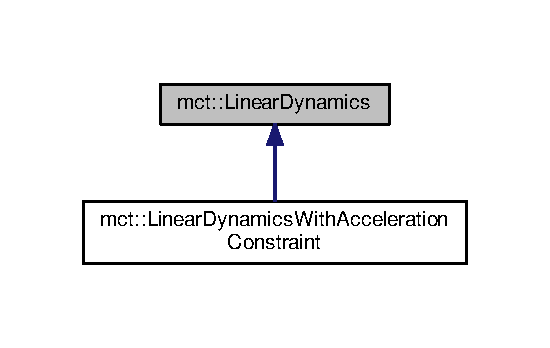
\includegraphics[width=264pt]{classmct_1_1LinearDynamics__inherit__graph}
\end{center}
\end{figure}
\subsection*{Public Types}
\begin{DoxyCompactItemize}
\item 
typedef Eigen\+::\+Matrix$<$ double, Eigen\+::\+Dynamic, 1, 0, 10 $>$ {\bfseries Vector}\hypertarget{classmct_1_1LinearDynamics_abd48cad5a3b6819e218cde41ec2670a0}{}\label{classmct_1_1LinearDynamics_abd48cad5a3b6819e218cde41ec2670a0}

\end{DoxyCompactItemize}
\subsection*{Public Member Functions}
\begin{DoxyCompactItemize}
\item 
{\bfseries Linear\+Dynamics} (Eigen\+::\+Vector4d parameters)\hypertarget{classmct_1_1LinearDynamics_a4cb41e128efc2d9fda1995610966da86}{}\label{classmct_1_1LinearDynamics_a4cb41e128efc2d9fda1995610966da86}

\item 
{\bfseries Linear\+Dynamics} (double jerk, double initial\+\_\+acceleration, double initial\+\_\+velocity, double initial\+\_\+position)\hypertarget{classmct_1_1LinearDynamics_a5c38619de6412eb2c85bb207fbe6d7ec}{}\label{classmct_1_1LinearDynamics_a5c38619de6412eb2c85bb207fbe6d7ec}

\item 
double {\bfseries get\+\_\+acceleration} (\hyperlink{classmct_1_1NonnegDouble}{mct\+::\+Nonneg\+Double} t) const \hypertarget{classmct_1_1LinearDynamics_a34d6238236aec2a1b30f66edc1e13db9}{}\label{classmct_1_1LinearDynamics_a34d6238236aec2a1b30f66edc1e13db9}

\item 
double {\bfseries get\+\_\+velocity} (\hyperlink{classmct_1_1NonnegDouble}{mct\+::\+Nonneg\+Double} t) const \hypertarget{classmct_1_1LinearDynamics_a0179d2a8a7adfb9280f5238d340e7534}{}\label{classmct_1_1LinearDynamics_a0179d2a8a7adfb9280f5238d340e7534}

\item 
double {\bfseries get\+\_\+position} (\hyperlink{classmct_1_1NonnegDouble}{mct\+::\+Nonneg\+Double} t) const \hypertarget{classmct_1_1LinearDynamics_a8896d67d7d8ecd3676ee1cc54041d03a}{}\label{classmct_1_1LinearDynamics_a8896d67d7d8ecd3676ee1cc54041d03a}

\item 
Vector {\bfseries find\+\_\+t\+\_\+given\+\_\+velocity} (double velocity) const \hypertarget{classmct_1_1LinearDynamics_ae0b39a3139d5f7de01ecbb6e66d85a6e}{}\label{classmct_1_1LinearDynamics_ae0b39a3139d5f7de01ecbb6e66d85a6e}

\end{DoxyCompactItemize}
\subsection*{Protected Attributes}
\begin{DoxyCompactItemize}
\item 
double {\bfseries jerk\+\_\+}\hypertarget{classmct_1_1LinearDynamics_aa12a81e1ef4e33e310bf02978a20fef4}{}\label{classmct_1_1LinearDynamics_aa12a81e1ef4e33e310bf02978a20fef4}

\item 
double {\bfseries initial\+\_\+acceleration\+\_\+}\hypertarget{classmct_1_1LinearDynamics_aa37dc8e527de707c9402b3de06e7e35f}{}\label{classmct_1_1LinearDynamics_aa37dc8e527de707c9402b3de06e7e35f}

\item 
double {\bfseries initial\+\_\+velocity\+\_\+}\hypertarget{classmct_1_1LinearDynamics_ab9db51c5442ac30a82f10fa33b3a024d}{}\label{classmct_1_1LinearDynamics_ab9db51c5442ac30a82f10fa33b3a024d}

\item 
double {\bfseries initial\+\_\+position\+\_\+}\hypertarget{classmct_1_1LinearDynamics_a4ab9e657e985729091d3136f98bb99fd}{}\label{classmct_1_1LinearDynamics_a4ab9e657e985729091d3136f98bb99fd}

\end{DoxyCompactItemize}


The documentation for this class was generated from the following file\+:\begin{DoxyCompactItemize}
\item 
include/mpi\+\_\+cpp\+\_\+tools/\hyperlink{dynamical__systems_8hpp}{dynamical\+\_\+systems.\+hpp}\end{DoxyCompactItemize}

\hypertarget{classmct_1_1LinearDynamicsWithAccelerationConstraint}{}\section{mct\+:\+:Linear\+Dynamics\+With\+Acceleration\+Constraint Class Reference}
\label{classmct_1_1LinearDynamicsWithAccelerationConstraint}\index{mct\+::\+Linear\+Dynamics\+With\+Acceleration\+Constraint@{mct\+::\+Linear\+Dynamics\+With\+Acceleration\+Constraint}}


Inheritance diagram for mct\+:\+:Linear\+Dynamics\+With\+Acceleration\+Constraint\+:
\nopagebreak
\begin{figure}[H]
\begin{center}
\leavevmode
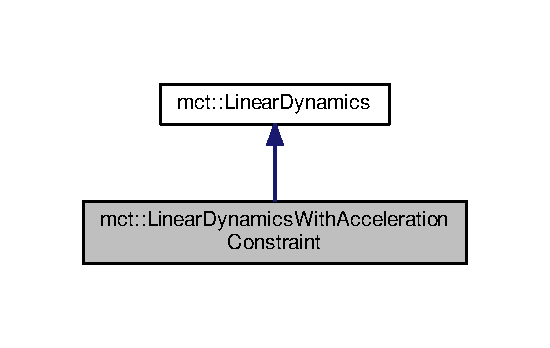
\includegraphics[width=264pt]{classmct_1_1LinearDynamicsWithAccelerationConstraint__inherit__graph}
\end{center}
\end{figure}


Collaboration diagram for mct\+:\+:Linear\+Dynamics\+With\+Acceleration\+Constraint\+:
\nopagebreak
\begin{figure}[H]
\begin{center}
\leavevmode
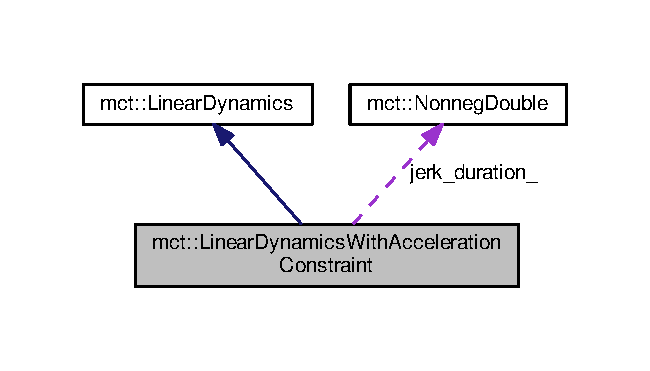
\includegraphics[width=312pt]{classmct_1_1LinearDynamicsWithAccelerationConstraint__coll__graph}
\end{center}
\end{figure}
\subsection*{Public Types}
\begin{DoxyCompactItemize}
\item 
typedef Linear\+Dynamics\+::\+Vector {\bfseries Vector}\hypertarget{classmct_1_1LinearDynamicsWithAccelerationConstraint_a9f31f3ecc820198a01eb0fc78c4dfb75}{}\label{classmct_1_1LinearDynamicsWithAccelerationConstraint_a9f31f3ecc820198a01eb0fc78c4dfb75}

\item 
typedef Eigen\+::\+Matrix$<$ double, Eigen\+::\+Dynamic, Eigen\+::\+Dynamic, 0, 10, 10 $>$ {\bfseries Matrix}\hypertarget{classmct_1_1LinearDynamicsWithAccelerationConstraint_a5a74321eebcdddebde9083145feb996f}{}\label{classmct_1_1LinearDynamicsWithAccelerationConstraint_a5a74321eebcdddebde9083145feb996f}

\end{DoxyCompactItemize}
\subsection*{Public Member Functions}
\begin{DoxyCompactItemize}
\item 
void {\bfseries print\+\_\+parameters} () const \hypertarget{classmct_1_1LinearDynamicsWithAccelerationConstraint_ade3a0d6eddf1a5af523270ae1fe13aca}{}\label{classmct_1_1LinearDynamicsWithAccelerationConstraint_ade3a0d6eddf1a5af523270ae1fe13aca}

\item 
{\bfseries Linear\+Dynamics\+With\+Acceleration\+Constraint} (Eigen\+::\+Matrix$<$ double, 5, 1 $>$ parameters)\hypertarget{classmct_1_1LinearDynamicsWithAccelerationConstraint_afe40d0fc5058e69055e0f4dbf59d611a}{}\label{classmct_1_1LinearDynamicsWithAccelerationConstraint_afe40d0fc5058e69055e0f4dbf59d611a}

\item 
{\bfseries Linear\+Dynamics\+With\+Acceleration\+Constraint} (double jerk, double initial\+\_\+acceleration, double initial\+\_\+velocity, double initial\+\_\+position, \hyperlink{classmct_1_1NonnegDouble}{mct\+::\+Nonneg\+Double} abs\+\_\+acceleration\+\_\+limit)\hypertarget{classmct_1_1LinearDynamicsWithAccelerationConstraint_a4501cf02cce687c60d6da0b24ef609d3}{}\label{classmct_1_1LinearDynamicsWithAccelerationConstraint_a4501cf02cce687c60d6da0b24ef609d3}

\item 
void {\bfseries set\+\_\+initial\+\_\+acceleration} (double initial\+\_\+acceleration)\hypertarget{classmct_1_1LinearDynamicsWithAccelerationConstraint_a8f9a83d5da9d9e7b9eb4031e43022dfe}{}\label{classmct_1_1LinearDynamicsWithAccelerationConstraint_a8f9a83d5da9d9e7b9eb4031e43022dfe}

\item 
double {\bfseries get\+\_\+acceleration} (\hyperlink{classmct_1_1NonnegDouble}{mct\+::\+Nonneg\+Double} t) const \hypertarget{classmct_1_1LinearDynamicsWithAccelerationConstraint_ad2691066026d0aa0e9c7867c98fc6685}{}\label{classmct_1_1LinearDynamicsWithAccelerationConstraint_ad2691066026d0aa0e9c7867c98fc6685}

\item 
double {\bfseries get\+\_\+velocity} (\hyperlink{classmct_1_1NonnegDouble}{mct\+::\+Nonneg\+Double} t) const \hypertarget{classmct_1_1LinearDynamicsWithAccelerationConstraint_a75b2c052e49a8b591b29df9551f05614}{}\label{classmct_1_1LinearDynamicsWithAccelerationConstraint_a75b2c052e49a8b591b29df9551f05614}

\item 
double {\bfseries get\+\_\+position} (\hyperlink{classmct_1_1NonnegDouble}{mct\+::\+Nonneg\+Double} t) const \hypertarget{classmct_1_1LinearDynamicsWithAccelerationConstraint_a79216cc4eef7308542d9811b8c44ecf6}{}\label{classmct_1_1LinearDynamicsWithAccelerationConstraint_a79216cc4eef7308542d9811b8c44ecf6}

\item 
{\footnotesize template$<$typename Array $>$ }\\Array {\bfseries get\+\_\+positions} (const Array \&times) const \hypertarget{classmct_1_1LinearDynamicsWithAccelerationConstraint_adaa181c2109d4f4098e7833e58ce929d}{}\label{classmct_1_1LinearDynamicsWithAccelerationConstraint_adaa181c2109d4f4098e7833e58ce929d}

\item 
Vector {\bfseries find\+\_\+t\+\_\+given\+\_\+velocity} (double velocity) const \hypertarget{classmct_1_1LinearDynamicsWithAccelerationConstraint_a9ce476e49904c83c85af67f5be5a5e2d}{}\label{classmct_1_1LinearDynamicsWithAccelerationConstraint_a9ce476e49904c83c85af67f5be5a5e2d}

\item 
bool {\bfseries will\+\_\+exceed\+\_\+jointly} (const double \&max\+\_\+velocity, const double \&max\+\_\+position) const \hypertarget{classmct_1_1LinearDynamicsWithAccelerationConstraint_a941585f2acda77a22a3a269ba6873afb}{}\label{classmct_1_1LinearDynamicsWithAccelerationConstraint_a941585f2acda77a22a3a269ba6873afb}

\item 
bool \hyperlink{classmct_1_1LinearDynamicsWithAccelerationConstraint_a568991a3b2459be274a86298caf8356c}{will\+\_\+exceed\+\_\+jointly} (const double \&max\+\_\+velocity, const double \&max\+\_\+position, double \&certificate\+\_\+time) const 
\item 
bool {\bfseries will\+\_\+deceed\+\_\+jointly} (const double \&min\+\_\+velocity, const double \&min\+\_\+position) const \hypertarget{classmct_1_1LinearDynamicsWithAccelerationConstraint_a9c94e5e278cb7519215a5495f326b11c}{}\label{classmct_1_1LinearDynamicsWithAccelerationConstraint_a9c94e5e278cb7519215a5495f326b11c}

\item 
bool {\bfseries will\+\_\+deceed\+\_\+jointly} (const double \&min\+\_\+velocity, const double \&min\+\_\+position, double \&certificate\+\_\+time) const \hypertarget{classmct_1_1LinearDynamicsWithAccelerationConstraint_ae3c5bef385c2bcb64b5a7cd9dae42654}{}\label{classmct_1_1LinearDynamicsWithAccelerationConstraint_ae3c5bef385c2bcb64b5a7cd9dae42654}

\end{DoxyCompactItemize}
\subsection*{Private Attributes}
\begin{DoxyCompactItemize}
\item 
double {\bfseries acceleration\+\_\+limit\+\_\+}\hypertarget{classmct_1_1LinearDynamicsWithAccelerationConstraint_a8030e84817471fde3716a5d4ea4f2927}{}\label{classmct_1_1LinearDynamicsWithAccelerationConstraint_a8030e84817471fde3716a5d4ea4f2927}

\item 
\hyperlink{classmct_1_1NonnegDouble}{mct\+::\+Nonneg\+Double} {\bfseries jerk\+\_\+duration\+\_\+}\hypertarget{classmct_1_1LinearDynamicsWithAccelerationConstraint_ad5f33b779d2503eca2a7bb1f53ccc0da}{}\label{classmct_1_1LinearDynamicsWithAccelerationConstraint_ad5f33b779d2503eca2a7bb1f53ccc0da}

\end{DoxyCompactItemize}
\subsection*{Additional Inherited Members}


\subsection{Member Function Documentation}
\index{mct\+::\+Linear\+Dynamics\+With\+Acceleration\+Constraint@{mct\+::\+Linear\+Dynamics\+With\+Acceleration\+Constraint}!will\+\_\+exceed\+\_\+jointly@{will\+\_\+exceed\+\_\+jointly}}
\index{will\+\_\+exceed\+\_\+jointly@{will\+\_\+exceed\+\_\+jointly}!mct\+::\+Linear\+Dynamics\+With\+Acceleration\+Constraint@{mct\+::\+Linear\+Dynamics\+With\+Acceleration\+Constraint}}
\subsubsection[{\texorpdfstring{will\+\_\+exceed\+\_\+jointly(const double \&max\+\_\+velocity, const double \&max\+\_\+position, double \&certificate\+\_\+time) const }{will_exceed_jointly(const double &max_velocity, const double &max_position, double &certificate_time) const }}]{\setlength{\rightskip}{0pt plus 5cm}bool mct\+::\+Linear\+Dynamics\+With\+Acceleration\+Constraint\+::will\+\_\+exceed\+\_\+jointly (
\begin{DoxyParamCaption}
\item[{const double \&}]{max\+\_\+velocity, }
\item[{const double \&}]{max\+\_\+position, }
\item[{double \&}]{certificate\+\_\+time}
\end{DoxyParamCaption}
) const\hspace{0.3cm}{\ttfamily [inline]}}\hypertarget{classmct_1_1LinearDynamicsWithAccelerationConstraint_a568991a3b2459be274a86298caf8356c}{}\label{classmct_1_1LinearDynamicsWithAccelerationConstraint_a568991a3b2459be274a86298caf8356c}
\begin{DoxyRefDesc}{Todo}
\item[\hyperlink{todo__todo000002}{Todo}]we could do this in a cleaner way with candidate points \end{DoxyRefDesc}


The documentation for this class was generated from the following file\+:\begin{DoxyCompactItemize}
\item 
include/mpi\+\_\+cpp\+\_\+tools/\hyperlink{dynamical__systems_8hpp}{dynamical\+\_\+systems.\+hpp}\end{DoxyCompactItemize}

\hypertarget{classmct_1_1NonnegDouble}{}\section{mct\+:\+:Nonneg\+Double Class Reference}
\label{classmct_1_1NonnegDouble}\index{mct\+::\+Nonneg\+Double@{mct\+::\+Nonneg\+Double}}
\subsection*{Public Member Functions}
\begin{DoxyCompactItemize}
\item 
{\bfseries Nonneg\+Double} (double value)\hypertarget{classmct_1_1NonnegDouble_a416aa156d31270f95b569b2e00cafa06}{}\label{classmct_1_1NonnegDouble_a416aa156d31270f95b569b2e00cafa06}

\item 
{\bfseries operator double} () const \hypertarget{classmct_1_1NonnegDouble_aabb3515195942147a8cd5e81a34331ca}{}\label{classmct_1_1NonnegDouble_aabb3515195942147a8cd5e81a34331ca}

\end{DoxyCompactItemize}
\subsection*{Private Attributes}
\begin{DoxyCompactItemize}
\item 
double {\bfseries value\+\_\+}\hypertarget{classmct_1_1NonnegDouble_a5129a6c7ffbd14b989523a210e8180e4}{}\label{classmct_1_1NonnegDouble_a5129a6c7ffbd14b989523a210e8180e4}

\end{DoxyCompactItemize}


The documentation for this class was generated from the following file\+:\begin{DoxyCompactItemize}
\item 
include/mpi\+\_\+cpp\+\_\+tools/\hyperlink{basic__tools_8hpp}{basic\+\_\+tools.\+hpp}\end{DoxyCompactItemize}

\hypertarget{classmct_1_1SafetyConstraint}{}\section{mct\+:\+:Safety\+Constraint Class Reference}
\label{classmct_1_1SafetyConstraint}\index{mct\+::\+Safety\+Constraint@{mct\+::\+Safety\+Constraint}}


Collaboration diagram for mct\+:\+:Safety\+Constraint\+:
\nopagebreak
\begin{figure}[H]
\begin{center}
\leavevmode
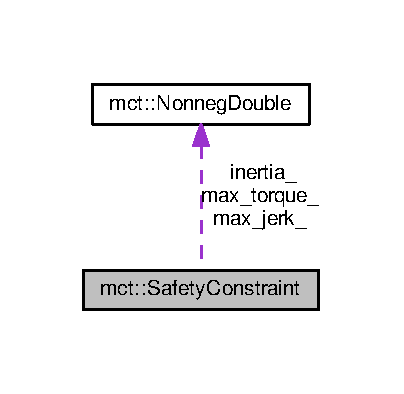
\includegraphics[width=194pt]{classmct_1_1SafetyConstraint__coll__graph}
\end{center}
\end{figure}
\subsection*{Public Member Functions}
\begin{DoxyCompactItemize}
\item 
{\bfseries Safety\+Constraint} (double min\+\_\+velocity, double min\+\_\+position, double max\+\_\+velocity, double max\+\_\+position, \hyperlink{classmct_1_1NonnegDouble}{mct\+::\+Nonneg\+Double} max\+\_\+torque, \hyperlink{classmct_1_1NonnegDouble}{mct\+::\+Nonneg\+Double} max\+\_\+jerk, \hyperlink{classmct_1_1NonnegDouble}{mct\+::\+Nonneg\+Double} inertia)\hypertarget{classmct_1_1SafetyConstraint_aaeed0e02691c4764e3a4934b8b42b69e}{}\label{classmct_1_1SafetyConstraint_aaeed0e02691c4764e3a4934b8b42b69e}

\item 
double {\bfseries get\+\_\+safe\+\_\+torque} (const double \&torque, const double \&velocity, const double \&position)\hypertarget{classmct_1_1SafetyConstraint_a8fbdcc71a00669057a8a957db41eea1e}{}\label{classmct_1_1SafetyConstraint_a8fbdcc71a00669057a8a957db41eea1e}

\end{DoxyCompactItemize}
\subsection*{Public Attributes}
\begin{DoxyCompactItemize}
\item 
double {\bfseries min\+\_\+velocity\+\_\+}\hypertarget{classmct_1_1SafetyConstraint_ae32fca1b6c738c3a3f101feb2fec5785}{}\label{classmct_1_1SafetyConstraint_ae32fca1b6c738c3a3f101feb2fec5785}

\item 
double {\bfseries min\+\_\+position\+\_\+}\hypertarget{classmct_1_1SafetyConstraint_afbec12a6f80368bb9e2b25de92dedcf2}{}\label{classmct_1_1SafetyConstraint_afbec12a6f80368bb9e2b25de92dedcf2}

\item 
double {\bfseries max\+\_\+velocity\+\_\+}\hypertarget{classmct_1_1SafetyConstraint_affeefa06a5a89e777f0779622cc21edc}{}\label{classmct_1_1SafetyConstraint_affeefa06a5a89e777f0779622cc21edc}

\item 
double {\bfseries max\+\_\+position\+\_\+}\hypertarget{classmct_1_1SafetyConstraint_a8b90d0a57f869e4cadec366aad397bcd}{}\label{classmct_1_1SafetyConstraint_a8b90d0a57f869e4cadec366aad397bcd}

\item 
\hyperlink{classmct_1_1NonnegDouble}{mct\+::\+Nonneg\+Double} {\bfseries max\+\_\+torque\+\_\+}\hypertarget{classmct_1_1SafetyConstraint_a9a7b128dcd64b5105f86d027b665ca02}{}\label{classmct_1_1SafetyConstraint_a9a7b128dcd64b5105f86d027b665ca02}

\item 
\hyperlink{classmct_1_1NonnegDouble}{mct\+::\+Nonneg\+Double} {\bfseries max\+\_\+jerk\+\_\+}\hypertarget{classmct_1_1SafetyConstraint_a0a50dbf6329aa075ba85fa60bd3b17dc}{}\label{classmct_1_1SafetyConstraint_a0a50dbf6329aa075ba85fa60bd3b17dc}

\item 
\hyperlink{classmct_1_1NonnegDouble}{mct\+::\+Nonneg\+Double} {\bfseries inertia\+\_\+}\hypertarget{classmct_1_1SafetyConstraint_affdcd5e2e62a8445fd02d83b7308fc6f}{}\label{classmct_1_1SafetyConstraint_affdcd5e2e62a8445fd02d83b7308fc6f}

\end{DoxyCompactItemize}


The documentation for this class was generated from the following file\+:\begin{DoxyCompactItemize}
\item 
include/mpi\+\_\+cpp\+\_\+tools/\hyperlink{dynamical__systems_8hpp}{dynamical\+\_\+systems.\+hpp}\end{DoxyCompactItemize}

\chapter{File Documentation}
\hypertarget{basic__tools_8hpp}{}\section{include/mpi\+\_\+cpp\+\_\+tools/basic\+\_\+tools.hpp File Reference}
\label{basic__tools_8hpp}\index{include/mpi\+\_\+cpp\+\_\+tools/basic\+\_\+tools.\+hpp@{include/mpi\+\_\+cpp\+\_\+tools/basic\+\_\+tools.\+hpp}}
{\ttfamily \#include $<$cmath$>$}\\*
Include dependency graph for basic\+\_\+tools.\+hpp\+:
\nopagebreak
\begin{figure}[H]
\begin{center}
\leavevmode
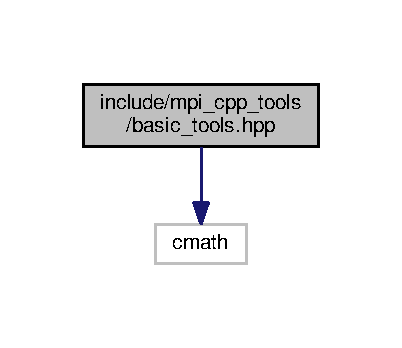
\includegraphics[width=193pt]{basic__tools_8hpp__incl}
\end{center}
\end{figure}
This graph shows which files directly or indirectly include this file\+:
\nopagebreak
\begin{figure}[H]
\begin{center}
\leavevmode
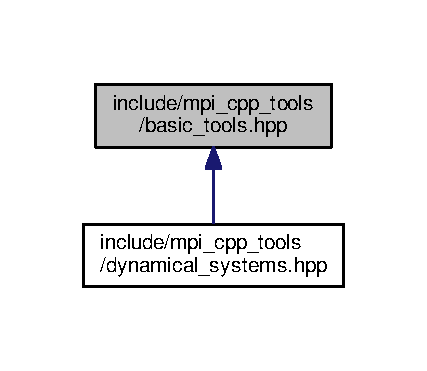
\includegraphics[width=205pt]{basic__tools_8hpp__dep__incl}
\end{center}
\end{figure}
\subsection*{Classes}
\begin{DoxyCompactItemize}
\item 
class \hyperlink{classmct_1_1NonnegDouble}{mct\+::\+Nonneg\+Double}
\end{DoxyCompactItemize}


\subsection{Detailed Description}
\begin{DoxyAuthor}{Author}
Manuel Wuthrich 
\end{DoxyAuthor}
\begin{DoxyRefDesc}{License}
\item[\hyperlink{license__license000001}{License}]License B\+S\+D-\/3-\/\+Clause \end{DoxyRefDesc}
\begin{DoxyCopyright}{Copyright}
Copyright (c) 2019, New York University and Max Planck Gesellschaft. 
\end{DoxyCopyright}
\begin{DoxyDate}{Date}
2019-\/08-\/05 
\end{DoxyDate}

\hypertarget{dynamical__systems_8hpp}{}\section{include/mpi\+\_\+cpp\+\_\+tools/dynamical\+\_\+systems.hpp File Reference}
\label{dynamical__systems_8hpp}\index{include/mpi\+\_\+cpp\+\_\+tools/dynamical\+\_\+systems.\+hpp@{include/mpi\+\_\+cpp\+\_\+tools/dynamical\+\_\+systems.\+hpp}}
{\ttfamily \#include $<$cmath$>$}\\*
{\ttfamily \#include $<$math.\+h$>$}\\*
{\ttfamily \#include $<$Eigen/\+Eigen$>$}\\*
{\ttfamily \#include $<$iostream$>$}\\*
{\ttfamily \#include \char`\"{}mpi\+\_\+cpp\+\_\+tools/basic\+\_\+tools.\+hpp\char`\"{}}\\*
{\ttfamily \#include \char`\"{}mpi\+\_\+cpp\+\_\+tools/math.\+hpp\char`\"{}}\\*
Include dependency graph for dynamical\+\_\+systems.\+hpp\+:
\nopagebreak
\begin{figure}[H]
\begin{center}
\leavevmode
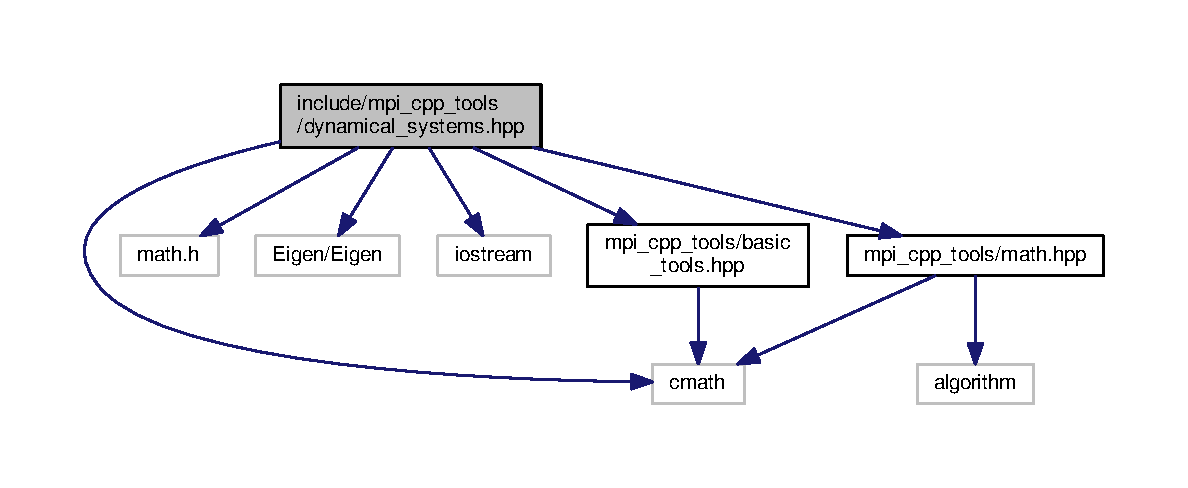
\includegraphics[width=350pt]{dynamical__systems_8hpp__incl}
\end{center}
\end{figure}
\subsection*{Classes}
\begin{DoxyCompactItemize}
\item 
class \hyperlink{classmct_1_1LinearDynamics}{mct\+::\+Linear\+Dynamics}
\item 
class \hyperlink{classmct_1_1LinearDynamicsWithAccelerationConstraint}{mct\+::\+Linear\+Dynamics\+With\+Acceleration\+Constraint}
\item 
class \hyperlink{classmct_1_1SafetyConstraint}{mct\+::\+Safety\+Constraint}
\end{DoxyCompactItemize}
\subsection*{Functions}
\begin{DoxyCompactItemize}
\item 
double \hyperlink{dynamical__systems_8hpp_aab449f0863dee56d0f0e377c75a4812d}{mct\+::find\+\_\+max\+\_\+admissible\+\_\+acceleration} (const double \&initial\+\_\+velocity, const double \&initial\+\_\+position, const double \&max\+\_\+velocity, const double \&max\+\_\+position, const \hyperlink{classmct_1_1NonnegDouble}{mct\+::\+Nonneg\+Double} \&abs\+\_\+jerk\+\_\+limit, const \hyperlink{classmct_1_1NonnegDouble}{mct\+::\+Nonneg\+Double} \&abs\+\_\+acceleration\+\_\+limit)
\item 
double {\bfseries mct\+::find\+\_\+min\+\_\+admissible\+\_\+acceleration} (const double \&initial\+\_\+velocity, const double \&initial\+\_\+position, const double \&min\+\_\+velocity, const double \&min\+\_\+position, const \hyperlink{classmct_1_1NonnegDouble}{mct\+::\+Nonneg\+Double} \&abs\+\_\+jerk\+\_\+limit, const \hyperlink{classmct_1_1NonnegDouble}{mct\+::\+Nonneg\+Double} \&abs\+\_\+acceleration\+\_\+limit)\hypertarget{dynamical__systems_8hpp_a87c8fdeac88fa24892ddb753f31f2a6c}{}\label{dynamical__systems_8hpp_a87c8fdeac88fa24892ddb753f31f2a6c}

\end{DoxyCompactItemize}


\subsection{Detailed Description}
\begin{DoxyAuthor}{Author}
Manuel Wuthrich 
\end{DoxyAuthor}
\begin{DoxyRefDesc}{License}
\item[\hyperlink{license__license000002}{License}]License B\+S\+D-\/3-\/\+Clause \end{DoxyRefDesc}
\begin{DoxyCopyright}{Copyright}
Copyright (c) 2019, New York University and Max Planck Gesellschaft. 
\end{DoxyCopyright}
\begin{DoxyDate}{Date}
2019-\/08-\/05 
\end{DoxyDate}


\subsection{Function Documentation}
\index{dynamical\+\_\+systems.\+hpp@{dynamical\+\_\+systems.\+hpp}!find\+\_\+max\+\_\+admissible\+\_\+acceleration@{find\+\_\+max\+\_\+admissible\+\_\+acceleration}}
\index{find\+\_\+max\+\_\+admissible\+\_\+acceleration@{find\+\_\+max\+\_\+admissible\+\_\+acceleration}!dynamical\+\_\+systems.\+hpp@{dynamical\+\_\+systems.\+hpp}}
\subsubsection[{\texorpdfstring{find\+\_\+max\+\_\+admissible\+\_\+acceleration(const double \&initial\+\_\+velocity, const double \&initial\+\_\+position, const double \&max\+\_\+velocity, const double \&max\+\_\+position, const mct\+::\+Nonneg\+Double \&abs\+\_\+jerk\+\_\+limit, const mct\+::\+Nonneg\+Double \&abs\+\_\+acceleration\+\_\+limit)}{find_max_admissible_acceleration(const double &initial_velocity, const double &initial_position, const double &max_velocity, const double &max_position, const mct::NonnegDouble &abs_jerk_limit, const mct::NonnegDouble &abs_acceleration_limit)}}]{\setlength{\rightskip}{0pt plus 5cm}double mct\+::find\+\_\+max\+\_\+admissible\+\_\+acceleration (
\begin{DoxyParamCaption}
\item[{const double \&}]{initial\+\_\+velocity, }
\item[{const double \&}]{initial\+\_\+position, }
\item[{const double \&}]{max\+\_\+velocity, }
\item[{const double \&}]{max\+\_\+position, }
\item[{const {\bf mct\+::\+Nonneg\+Double} \&}]{abs\+\_\+jerk\+\_\+limit, }
\item[{const {\bf mct\+::\+Nonneg\+Double} \&}]{abs\+\_\+acceleration\+\_\+limit}
\end{DoxyParamCaption}
)}\hypertarget{dynamical__systems_8hpp_file_aab449f0863dee56d0f0e377c75a4812d}{}\label{dynamical__systems_8hpp_file_aab449f0863dee56d0f0e377c75a4812d}
\begin{DoxyRefDesc}{Todo}
\item[\hyperlink{todo__todo000001}{Todo}]\+: not quite sure what is the right thing to do here \end{DoxyRefDesc}

\hypertarget{math_8hpp}{}\section{include/mpi\+\_\+cpp\+\_\+tools/math.hpp File Reference}
\label{math_8hpp}\index{include/mpi\+\_\+cpp\+\_\+tools/math.\+hpp@{include/mpi\+\_\+cpp\+\_\+tools/math.\+hpp}}
{\ttfamily \#include $<$cmath$>$}\\*
{\ttfamily \#include $<$algorithm$>$}\\*
Include dependency graph for math.\+hpp\+:
\nopagebreak
\begin{figure}[H]
\begin{center}
\leavevmode
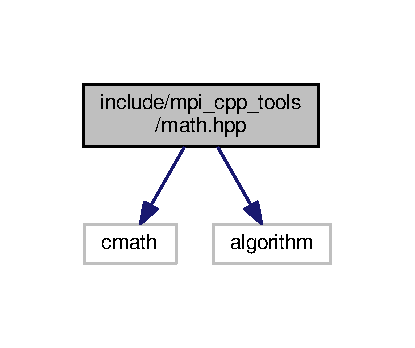
\includegraphics[width=199pt]{math_8hpp__incl}
\end{center}
\end{figure}
This graph shows which files directly or indirectly include this file\+:
\nopagebreak
\begin{figure}[H]
\begin{center}
\leavevmode
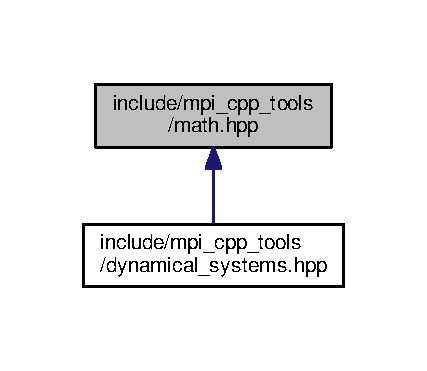
\includegraphics[width=205pt]{math_8hpp__dep__incl}
\end{center}
\end{figure}
\subsection*{Functions}
\begin{DoxyCompactItemize}
\item 
double {\bfseries mct\+::clamp} (const double \&value, const double \&limit\+\_\+a, const double \&limit\+\_\+b)\hypertarget{math_8hpp_acee1bab6012500f4f6709fadef426407}{}\label{math_8hpp_acee1bab6012500f4f6709fadef426407}

\item 
{\footnotesize template$<$typename Vector $>$ }\\Vector {\bfseries mct\+::clamp} (const Vector \&vector, const double \&limit\+\_\+a, const double \&limit\+\_\+b)\hypertarget{math_8hpp_a0da0a10ac9a5f53e1bff7004b9375ef1}{}\label{math_8hpp_a0da0a10ac9a5f53e1bff7004b9375ef1}

\item 
{\footnotesize template$<$typename Vector $>$ }\\void {\bfseries mct\+::append\+\_\+to\+\_\+vector} (Vector \&vector, const double \&element)\hypertarget{math_8hpp_a51a2b8ea864671201f79d50310a0cdd4}{}\label{math_8hpp_a51a2b8ea864671201f79d50310a0cdd4}

\item 
{\footnotesize template$<$typename Matrix $>$ }\\void {\bfseries mct\+::append\+\_\+rows\+\_\+to\+\_\+matrix} (Matrix \&matrix, const Matrix \&rows)\hypertarget{math_8hpp_aab77f23043c1849bee062cf75c75d101}{}\label{math_8hpp_aab77f23043c1849bee062cf75c75d101}

\item 
bool {\bfseries mct\+::approx\+\_\+equal} (double x, double y, double epsilon=1e-\/10)\hypertarget{math_8hpp_a6014d19d6c69a7a98aac6b68c57e6795}{}\label{math_8hpp_a6014d19d6c69a7a98aac6b68c57e6795}

\item 
{\footnotesize template$<$typename Vector $>$ }\\bool {\bfseries mct\+::contains} (Vector v, double x)\hypertarget{math_8hpp_a1cee0ed64de57025bf7ab0ae767008e6}{}\label{math_8hpp_a1cee0ed64de57025bf7ab0ae767008e6}

\end{DoxyCompactItemize}


\subsection{Detailed Description}
\begin{DoxyAuthor}{Author}
Manuel Wuthrich 
\end{DoxyAuthor}
\begin{DoxyRefDesc}{License}
\item[\hyperlink{license__license000003}{License}]License B\+S\+D-\/3-\/\+Clause \end{DoxyRefDesc}
\begin{DoxyCopyright}{Copyright}
Copyright (c) 2019, New York University and Max Planck Gesellschaft. 
\end{DoxyCopyright}
\begin{DoxyDate}{Date}
2019-\/08-\/05 
\end{DoxyDate}

%--- End generated contents ---

% Index
\backmatter
\newpage
\phantomsection
\clearemptydoublepage
\addcontentsline{toc}{chapter}{Index}
\printindex

\end{document}
